\subsection{Admin view}
    \noindent 
    \begin{minipage}{0.5\textwidth}
        \vspace{1cm}
        \fbox{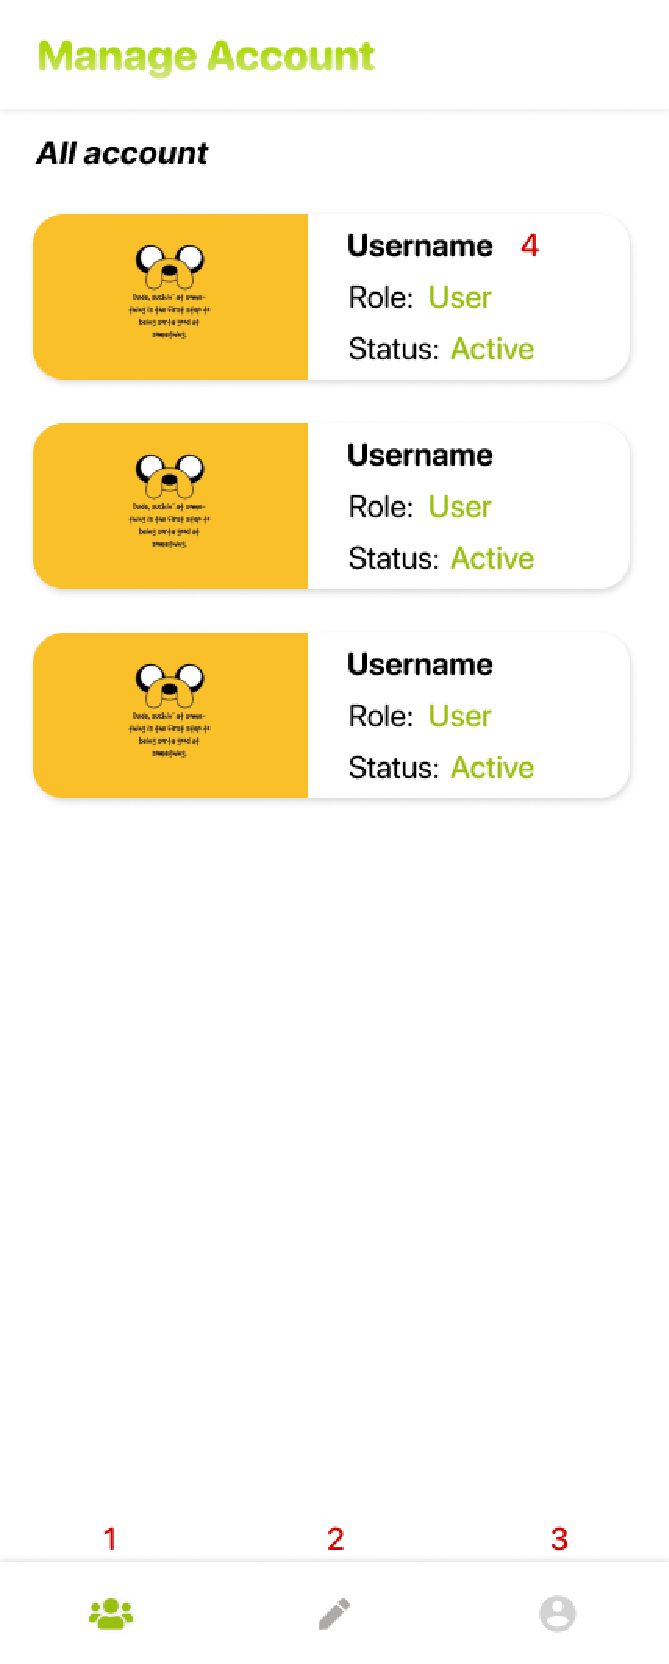
\includegraphics[width=\textwidth]{images/ui/Manage account.pdf}}
        \captionof{figure}{Trang quản lý tài khoản}
    \end{minipage}
    \hspace{0.05\textwidth}
    \begin{minipage}{0.45\textwidth}
        \begin{tblr}{
            width=1\linewidth,
            hlines, 
            vlines,
            colspec={X[1]X[2]X[7]},
            columns = {valign = m, },
            column{1} = {halign = c},
            row{1} = {halign = c, valign = m, bg = lightgray, fg = black},
            }
            {\textbf{\#}} & \textbf{Type} & {\textbf{Mô tả}} \\
            1 & Button & Chuyển tới trang quản lý tài khoản\\
            2 & Button &  Chuyển tới trang quản lý món ăn\\
            3 & Button & Chuyển đến trang thông tin cá nhân\\
            4 & Link & Chuyển đến trang thông tin tài khoản chi tiết\\
        \end{tblr}
    \end{minipage}
    
    \noindent 
    \begin{minipage}{0.5\textwidth}
        \vspace{1cm}
        \fbox{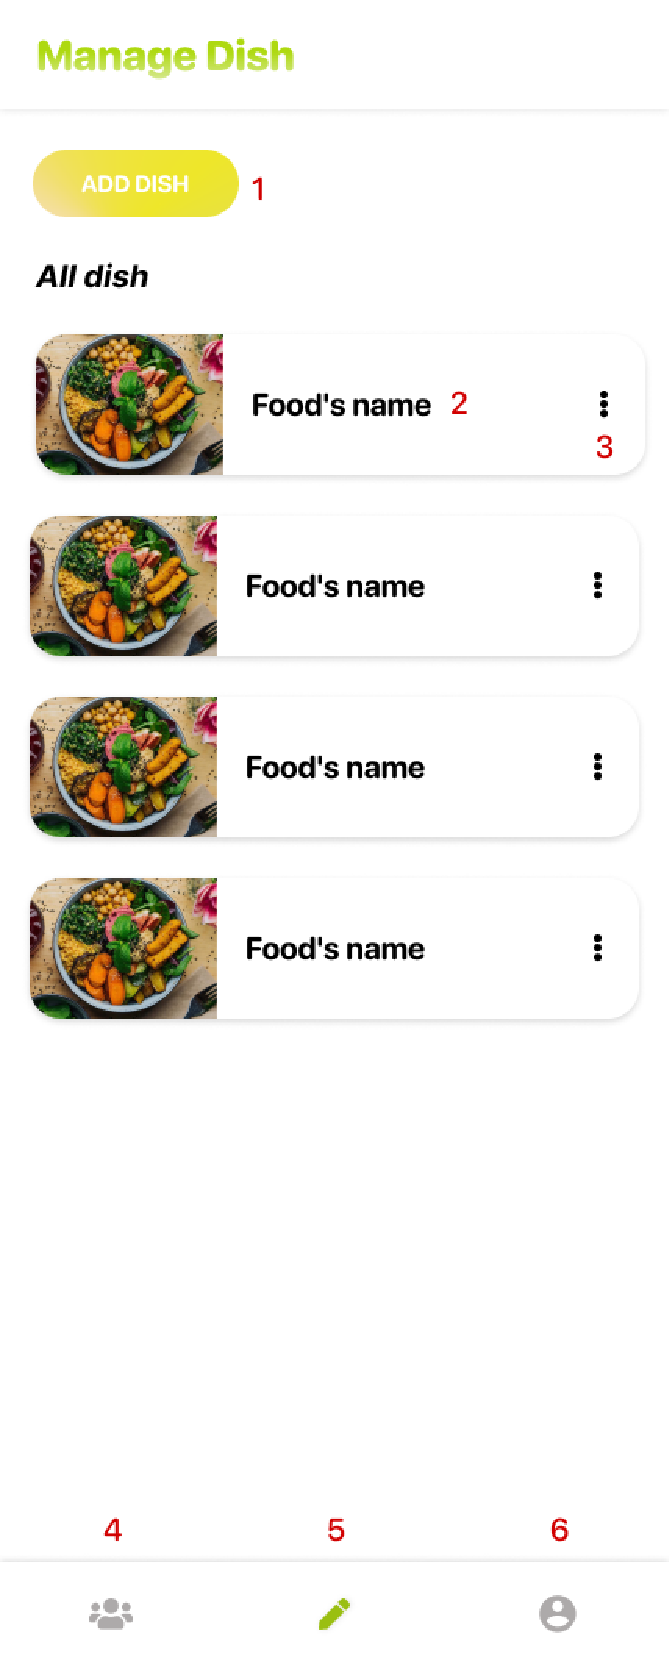
\includegraphics[width=\textwidth]{images/ui/Manage dish.pdf}}
        \captionof{figure}{Trang quản lý món ăn}
    \end{minipage}
    \hspace{0.05\textwidth}
    \begin{minipage}{0.45\textwidth}
        \begin{tblr}{
            width=1\linewidth,
            hlines, 
            vlines,
            colspec={X[1]X[2]X[7]},
            columns = {valign = m, },
            column{1} = {halign = c},
            row{1} = {halign = c, valign = m, bg = lightgray, fg = black},
            }
            {\textbf{\#}} & \textbf{Type} & {\textbf{Mô tả}} \\
            1 & Button & Chuyển tới trang tạo món ăn mới\\
            2 & Link &  Chuyển tới trang thông tin món ăn\\
            3 & Button & Hiển thị các tùy chọn cho món ăn \\
            4 & Button & Chuyển tới trang quản lý tài khoản \\
            5 & Button &  Chuyển tới trang quản lý món ăn\\
            6 & Button & Chuyển đến trang thông tin cá nhân\\
        \end{tblr}
    \end{minipage}
    
    \noindent 
    \begin{minipage}{0.5\textwidth}
        \vspace{1cm}
        \fbox{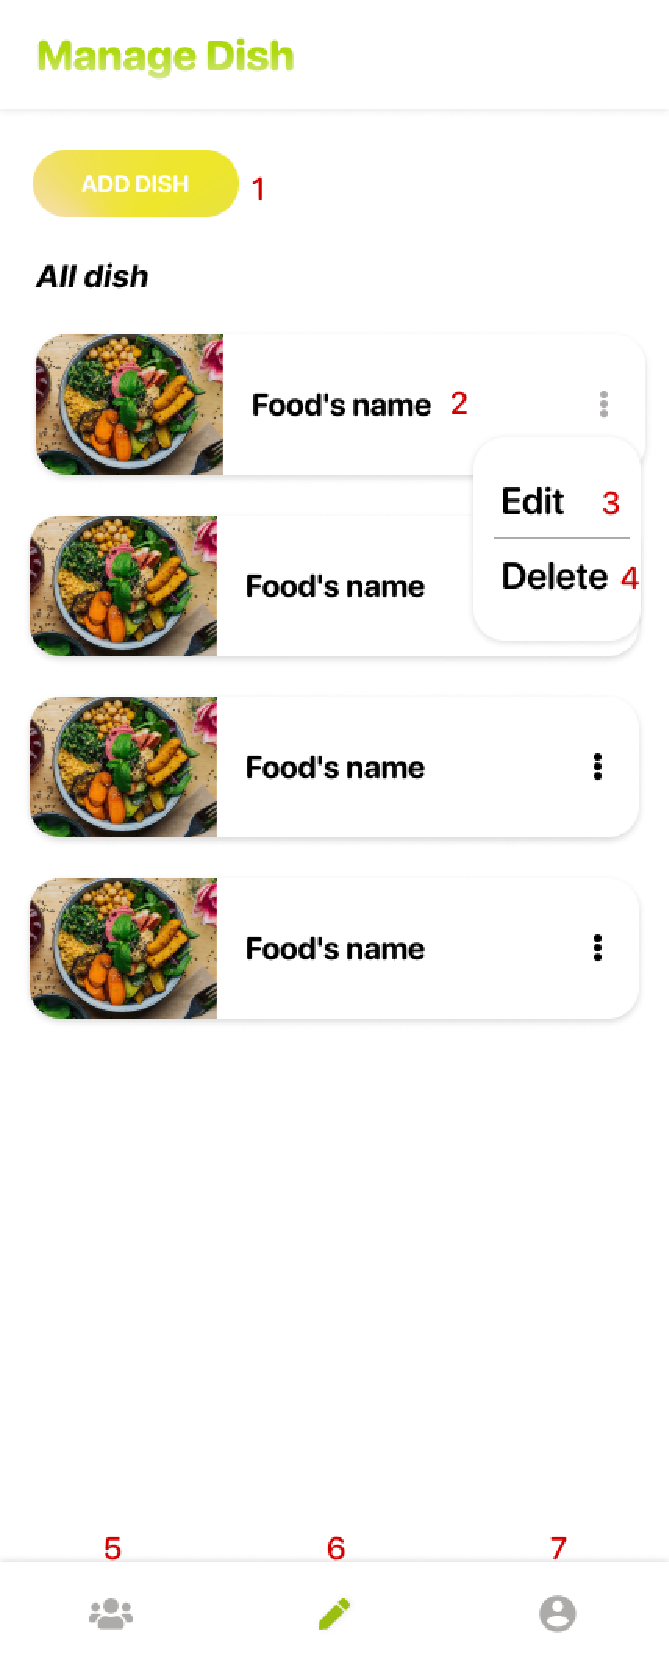
\includegraphics[width=\textwidth]{images/ui/Manage dish - submenu.pdf}}
        \captionof{figure}{Trang quản lý món ăn (tùy chọn)}
    \end{minipage}
    \hspace{0.05\textwidth}
    \begin{minipage}{0.45\textwidth}
        \begin{tblr}{
            width=1\linewidth,
            hlines, 
            vlines,
            colspec={X[1]X[2]X[7]},
            columns = {valign = m, },
            column{1} = {halign = c},
            row{1} = {halign = c, valign = m, bg = lightgray, fg = black},
            }
            {\textbf{\#}} & \textbf{Type} & {\textbf{Mô tả}} \\
            1 & Button & Chuyển tới trang tạo món ăn mới\\
            2 & Link &  Chuyển tới trang thông tin món ăn\\
            3 & Button & Chuyển tới trang chỉnh sửa món ăn \\
            4 & Button & Xóa món ăn, thông báo xác nhận hiển thị \\
            5 & Button & Chuyển tới trang quản lý tài khoản \\
            6 & Button &  Chuyển tới trang quản lý món ăn\\
            7 & Button & Chuyển đến trang thông tin cá nhân\\
        \end{tblr}
    \end{minipage}
    
    \noindent 
    \begin{minipage}{0.5\textwidth}
        \vspace{1cm}
        \fbox{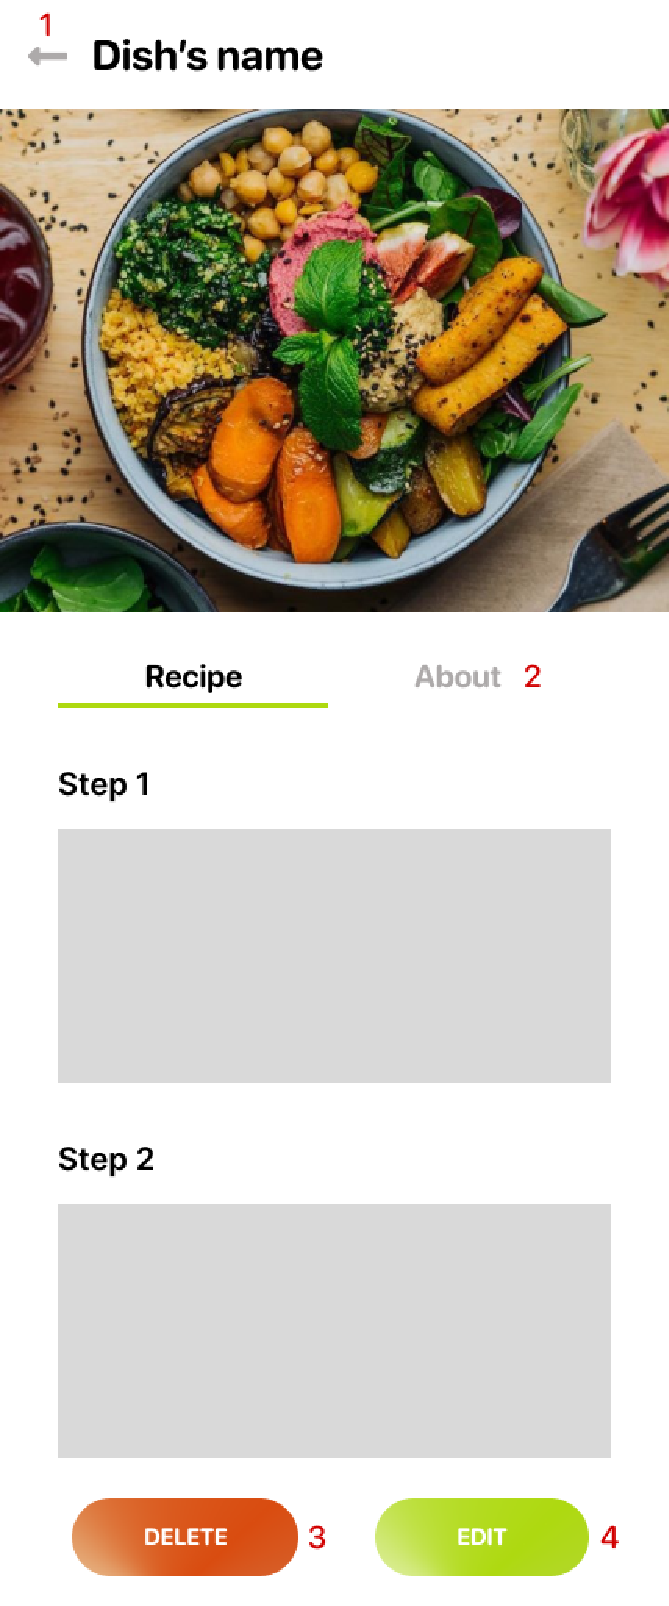
\includegraphics[width=\textwidth]{images/ui/Dish detail - manage - 1.pdf}}
        \captionof{figure}{Trang thông tin món ăn (Công thức)}
    \end{minipage}
    \hspace{0.05\textwidth}
    \begin{minipage}{0.45\textwidth}
        \begin{tblr}{
            width=1\linewidth,
            hlines, 
            vlines,
            colspec={X[1]X[2]X[7]},
            columns = {valign = m, },
            column{1} = {halign = c},
            row{1} = {halign = c, valign = m, bg = lightgray, fg = black},
            }
            {\textbf{\#}} & \textbf{Type} & {\textbf{Mô tả}} \\
            1 & Button & Quay lại trang quản lý món ăn\\
            2 & Button & Chuyển sang tab thông tin\\
            3 & Button & Xóa món ăn, thông báo xác nhận hiển thị \\
            4 & Button & Chuyển tới trang chỉnh sửa món ăn \\
        \end{tblr}
    \end{minipage}
    
    \noindent 
    \begin{minipage}{0.5\textwidth}
        \vspace{1cm}
        \fbox{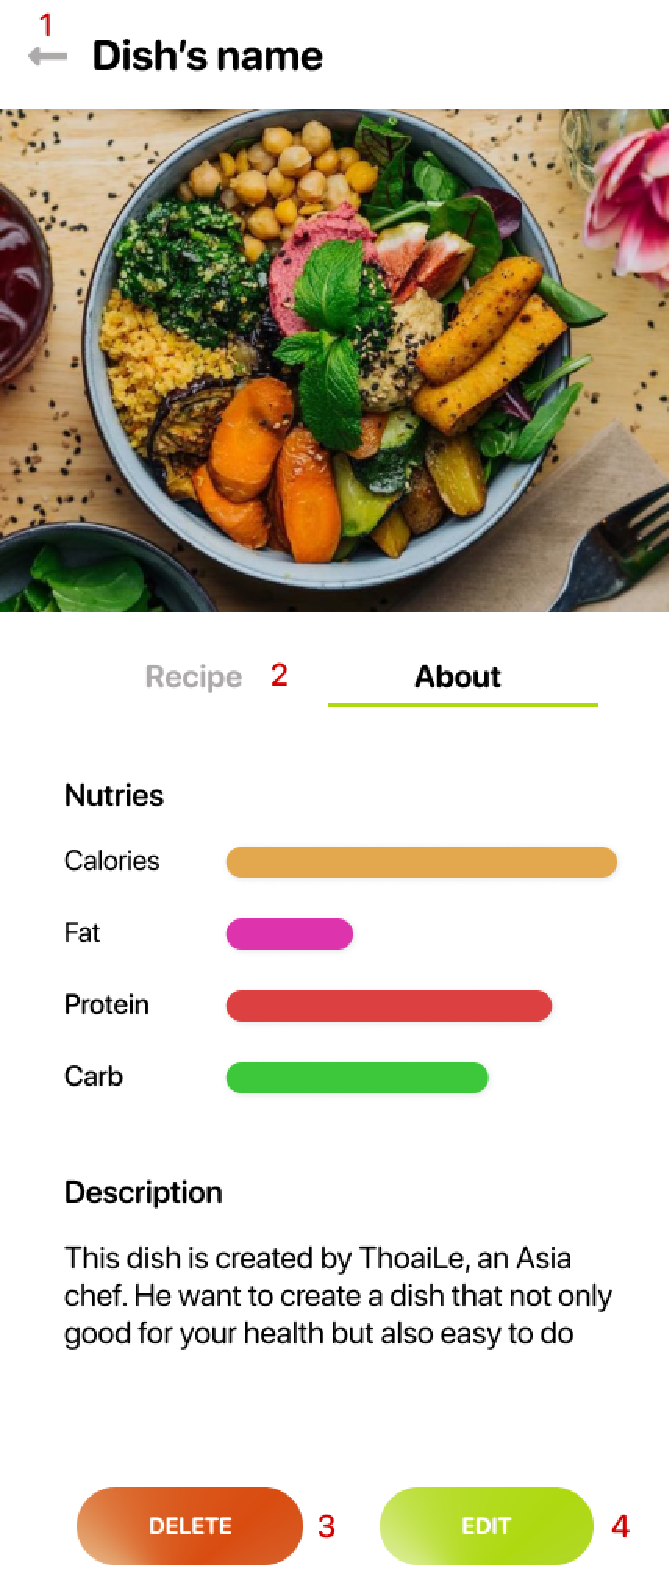
\includegraphics[width=\textwidth]{images/ui/Dish detail - manage - 2.pdf}}
        \captionof{figure}{Trang thông tin món ăn (Thông tin)}
    \end{minipage}
    \hspace{0.05\textwidth}
    \begin{minipage}{0.45\textwidth}
        \begin{tblr}{
            width=1\linewidth,
            hlines, 
            vlines,
            colspec={X[1]X[2]X[7]},
            columns = {valign = m, },
            column{1} = {halign = c},
            row{1} = {halign = c, valign = m, bg = lightgray, fg = black},
            }
            {\textbf{\#}} & \textbf{Type} & {\textbf{Mô tả}} \\
            1 & Button & Quay lại trang quản lý món ăn\\
            2 & Button & Chuyển sang tab công thức\\
            3 & Button & Xóa món ăn, thông báo xác nhận hiển thị \\
            4 & Button & Chuyển tới trang chỉnh sửa món ăn \\
        \end{tblr}
    \end{minipage}
    
    \noindent 
    \begin{minipage}{0.5\textwidth}
        \vspace{1cm}
        \fbox{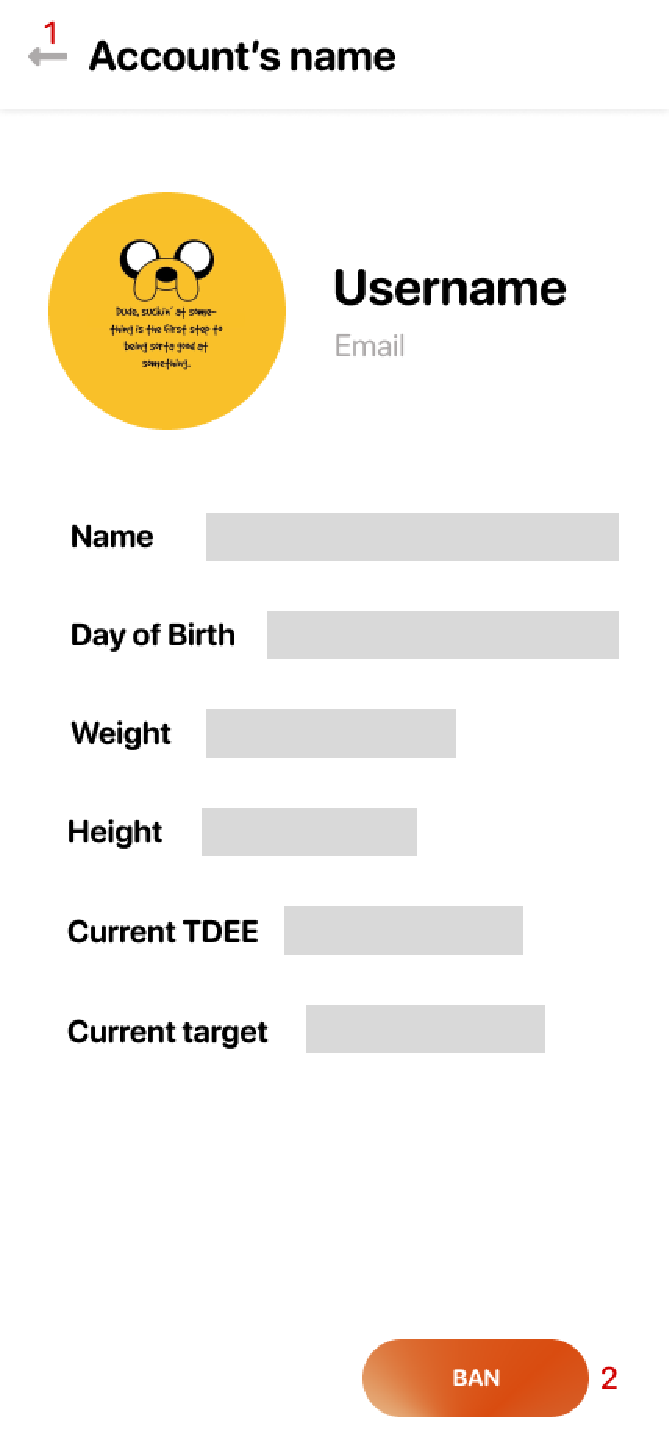
\includegraphics[width=\textwidth]{images/ui/Account detail - manage.pdf}}
        \captionof{figure}{Trang thông tin tài khoản}
    \end{minipage}
    \hspace{0.05\textwidth}
    \begin{minipage}{0.45\textwidth}
        \begin{tblr}{
            width=1\linewidth,
            hlines, 
            vlines,
            colspec={X[1]X[2]X[7]},
            columns = {valign = m, },
            column{1} = {halign = c},
            row{1} = {halign = c, valign = m, bg = lightgray, fg = black},
            }
            {\textbf{\#}} & \textbf{Type} & {\textbf{Mô tả}} \\
            1 & Button & Quay lại trang quản lý tài khoản\\
            2 & Button & Xác nhận cấm tài khoản\\
        \end{tblr}
    \end{minipage}
    
    \noindent 
    \begin{minipage}{0.5\textwidth}
        \vspace{1cm}
        \fbox{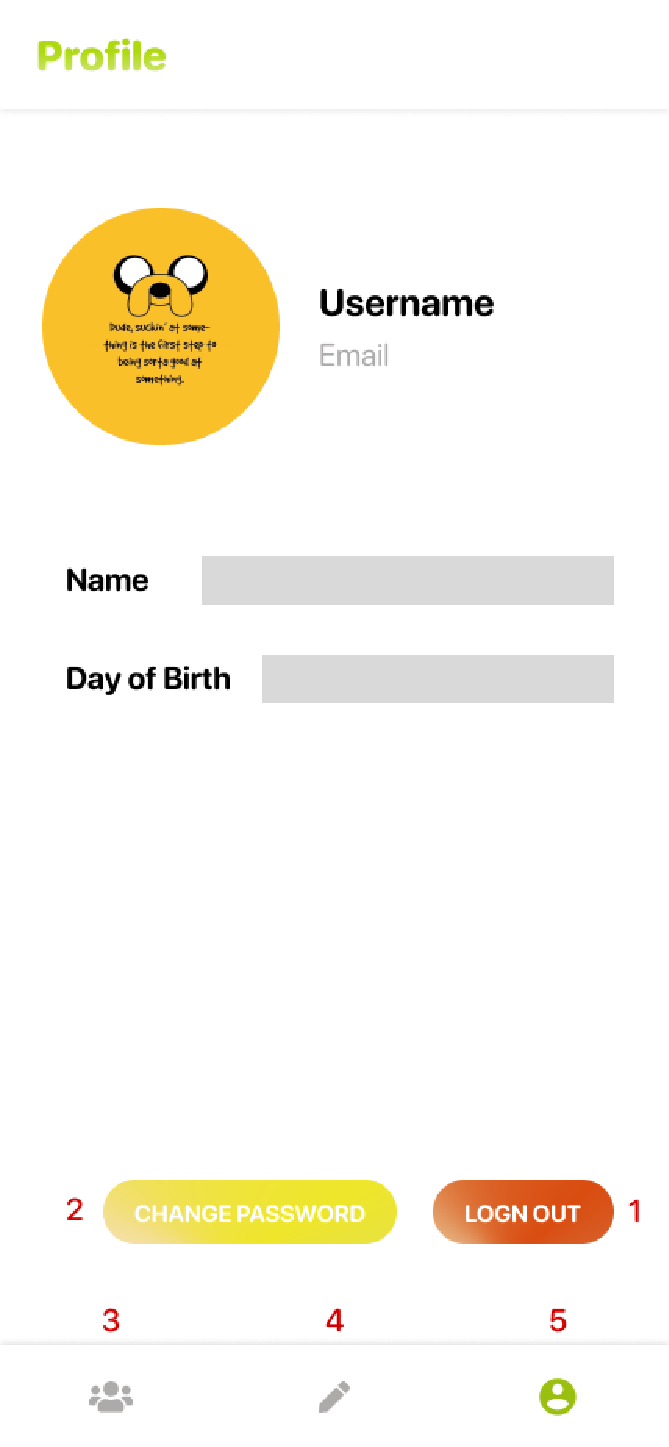
\includegraphics[width=\textwidth]{images/ui/Profile - admin.pdf}}
        \captionof{figure}{Trang thông cá nhân}
    \end{minipage}
    \hspace{0.05\textwidth}
    \begin{minipage}{0.45\textwidth}
        \begin{tblr}{
            width=1\linewidth,
            hlines, 
            vlines,
            colspec={X[1]X[2]X[7]},
            columns = {valign = m, },
            column{1} = {halign = c},
            row{1} = {halign = c, valign = m, bg = lightgray, fg = black},
            }
            {\textbf{\#}} & \textbf{Type} & {\textbf{Mô tả}} \\
            1 & Button & Đăng xuất, quay lại trang đăng nhập\\
            2 & Button & Chuyển tới trang đổi mật khẩu \\
            3 & Button & Chuyển tới trang quản lý tài khoản \\
            4 & Button &  Chuyển tới trang quản lý món ăn\\
            5 & Button & Chuyển đến trang thông tin cá nhân\\
        \end{tblr}
    \end{minipage}
    
    \noindent 
    \begin{minipage}{0.5\textwidth}
    	\vspace{1cm}
    	\fbox{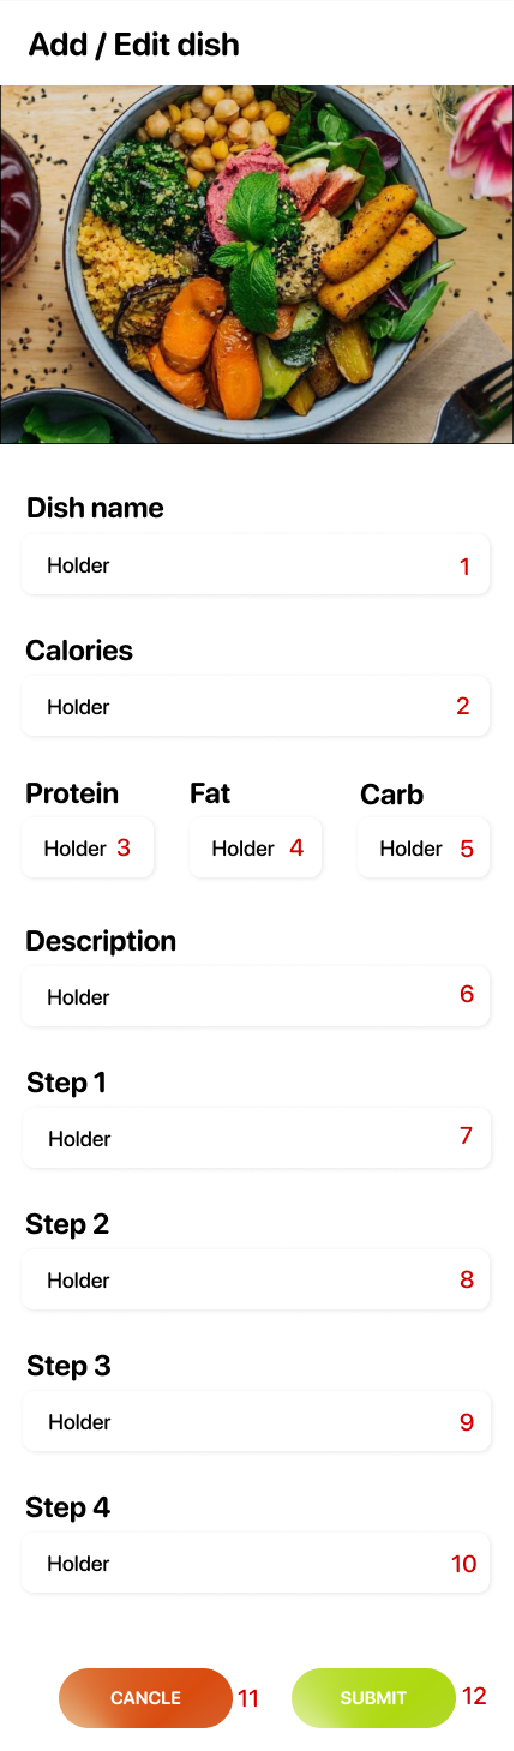
\includegraphics[width=0.7\textwidth]{images/ui/Edit dish.pdf}}
    	\captionof{figure}{Thêm / chỉnh sửa món ăn}
    \end{minipage}
    \hspace{0.05\textwidth}
    \begin{minipage}{0.45\textwidth}
    	\begin{tblr}{
    			width=1\linewidth,
    			hlines, 
    			vlines,
    			colspec={X[2]X[2]X[6]},
    			columns = {valign = m, },
    			column{1} = {halign = c},
    			row{1} = {halign = c, valign = m, bg = lightgray, fg = black},
    		}
    		{\textbf{\#}} & \textbf{Type} & {\textbf{Mô tả}} \\
    		1 & Input & Nhập tên món ăn\\
    		2 & Input & Nhập calories món ăn\\
    		3, 4, 5 & Input & Nhập Protein, Fat, Carb món ăn \\
    		6 & Input & Nhập mô tả món ăn \\
    		7, 8, 9, 10 & Input & Nhập từng bước nấu món ăn \\
    		11 & Button & Hủy thêm món ăn, quay lại trang quản lý món ăn \\
    		12 & Button & Xác nhận thêm món ăn, hệ thống lưu món ăn, quay lại trang quản lý món ăn \\
    	\end{tblr}
    \end{minipage}
    
    \noindent 
    \begin{minipage}{0.5\textwidth}
        \vspace{1cm}
        \fbox{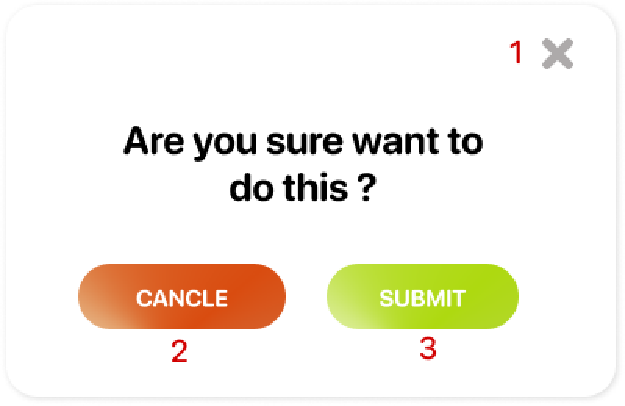
\includegraphics[width=\textwidth]{images/ui/Warning.pdf}}
        \captionof{figure}{Xác nhận xóa món ăn}
    \end{minipage}
    \hspace{0.05\textwidth}
    \begin{minipage}{0.45\textwidth}
        \begin{tblr}{
            width=1\linewidth,
            hlines, 
            vlines,
            colspec={X[1]X[2]X[7]},
            columns = {valign = m, },
            column{1} = {halign = c},
            row{1} = {halign = c, valign = m, bg = lightgray, fg = black},
            }
            {\textbf{\#}} & \textbf{Type} & {\textbf{Mô tả}} \\
            1 & Button & Hủy, đóng bảng thông báo\\
            2 & Button & Hủy, đóng bảng thông báo \\
            3 & Button & Xác nhân, đóng bản thông báo, món ăn bị xóa \\
        \end{tblr}
    \end{minipage}
